% =====================================================================
%  Beamer presentation — Women in Logic
%  Fuzzifying Derivatives of Regular Expressions
%  Mariam Katamashvili et al.  Kutaisi International University, 2026.
%
%  Build:
%      latexmk presentation.tex      % lualatex via .latexmkrc
%  or  lualatex presentation.tex
%
%  Slides are deliberately terse; the talking points live in script.txt.
%  The automaton on the "Constructing the automaton" frame is built one
%  state/edge per click (Beamer overlays).
% =====================================================================
\documentclass[aspectratio=169]{beamer}

% ---- Theme -----------------------------------------------------------
\usetheme{Madrid}
\usecolortheme{default}
\setbeamertemplate{navigation symbols}{}

% ---- Cold purple palette (replaces Madrid's default blue) ------------
\definecolor{coldpurple}{RGB}{74,45,140}      % base
\definecolor{coldpurplemid}{RGB}{108,80,175}  % medium
\definecolor{coldpurplelt}{RGB}{150,128,205}  % light
\definecolor{verifiedteal}{RGB}{20,120,100}   % "machine-checked"
\definecolor{ongoingamber}{RGB}{176,120,20}   % "ongoing / on paper"

\setbeamercolor{structure}{fg=coldpurple}
\setbeamercolor{palette primary}{bg=coldpurple,fg=white}
\setbeamercolor{palette secondary}{bg=coldpurplemid,fg=white}
\setbeamercolor{palette tertiary}{bg=coldpurplelt,fg=white}
\setbeamercolor{frametitle}{bg=coldpurple,fg=white}
\setbeamercolor{title}{bg=coldpurple,fg=white}
\setbeamercolor{block title}{bg=coldpurplemid,fg=white}
\setbeamercolor{block body}{bg=coldpurplelt!18,fg=black}
\setbeamercolor{alerted text}{fg=coldpurple}
\setbeamertemplate{itemize items}[circle]

% ---- Fonts / encoding ------------------------------------------------
\usepackage[T1]{fontenc}
\usepackage[utf8]{inputenc}
\usepackage{lmodern}

% ---- Packages --------------------------------------------------------
\usepackage{amsmath, amssymb, amsthm}
\usepackage{mathtools}
\usepackage{booktabs}
\usepackage{listings}
\usepackage{xcolor}
\usepackage{pifont}
\usepackage{tikz}
\usetikzlibrary{automata,positioning,arrows.meta,overlay-beamer-styles}

% ---- Shorthand macros (mirroring the paper) --------------------------
\newcommand{\cR}{\mathcal{R}}
\newcommand{\cut}{\mu}
\newcommand{\Dd}{\mathcal{D}}                 % syntactic derivative
\newcommand{\eps}{\varepsilon}
\newcommand{\st}{^{*}}                         % Kleene star
\newcommand{\tagcheck}{{\footnotesize\textcolor{verifiedteal}{\ding{51}\,Rocq-checked}}}
\newcommand{\tagpaper}{{\footnotesize\textcolor{ongoingamber}{\ding{119}\,on paper}}}

% ---- Rocq code listing style -----------------------------------------
\definecolor{rocqkw}{RGB}{140,20,20}
\definecolor{rocqcmt}{RGB}{60,120,60}
\definecolor{rocqbg}{RGB}{248,248,248}
\lstdefinestyle{rocqstyle}{
  basicstyle=\ttfamily\scriptsize,
  keywordstyle=\color{rocqkw}\bfseries,
  commentstyle=\color{rocqcmt}\itshape,
  backgroundcolor=\color{rocqbg},
  frame=single,
  rulecolor=\color{gray!40},
  breaklines=true,
  columns=fullflexible,
  keepspaces=true,
  showstringspaces=false,
  morekeywords={Definition,Fixpoint,Inductive,Theorem,Lemma,Proof,Qed,
    match,with,end,fun,forall,exists,Type,Prop,Set,let,in,if,then,else,
    Notation,Record,Structure,Class,Instance,elim,rewrite,by}
}

% ---- Section divider frames ------------------------------------------
\setbeamercolor{section in toc}{fg=coldpurple}
\setbeamercolor{section in toc shaded}{fg=black!35}
\AtBeginSection[]{%
  \begin{frame}{Where we are}
    \tableofcontents[currentsection,sectionstyle=show/shaded]
  \end{frame}
}

% ---- Title metadata --------------------------------------------------
\title[Fuzzifying Derivatives]{Fuzzifying Derivatives of\\Regular Expressions}
\subtitle{Women in Logic, FLoC 2026}
\author[Katamashvili, Maisuradze]{Mariam Katamashvili \and David Maisuradze}
\institute[VIAM, KIU]{Kutaisi International University \\ Vekua Institute of Applied Mathematics, TSU}
\date{2026}

% =====================================================================
\begin{document}

% ---- Title frame -----------------------------------------------------
\begin{frame}
  \titlepage
\end{frame}

% ---- Outline ---------------------------------------------------------
\begin{frame}{Outline}
  \tableofcontents
\end{frame}

% =====================================================================
\section{Derivatives}

\begin{frame}{Running a regular expression}
  To test whether a word matches a pattern, we have to \emph{run} the pattern on
  the word. There is more than one way to do this.
  \vfill
  \begin{columns}[T,onlytextwidth]
    \begin{column}{0.48\textwidth}
      \textbf{Compile to an automaton}
      \medskip

      Turn the pattern into a separate machine, then feed the word to it. The
      classical route: Thompson, Glushkov, the subset construction.
    \end{column}
    \begin{column}{0.48\textwidth}
      \textbf{Differentiate the pattern}
      \medskip

      Never build a machine. The \textbf{derivative} is what is left to match
      after reading a symbol; one derivative per symbol runs the pattern.
    \end{column}
  \end{columns}
  \vfill
  \begin{block}{We take the second route}
    And, as we will see, differentiating a pattern hands us the automaton
    anyway.
  \end{block}
\end{frame}

\begin{frame}{The derivative of a regular expression}
  The derivative $\Dd_a(r)$ is what remains to be matched once we have read the
  symbol $a$. On languages it simply strips a leading $a$:
  \[
    \partial_a(L)=\{\, w \mid a\cdot w\in L \,\}.
  \]
  On expressions it is computed directly, by recursion on the syntax:
  \[
  \begin{array}{rcl@{\qquad\qquad\qquad}rcl}
    \Dd_a(\emptyset) &=& \emptyset, & \Dd_a(r{+}s) &=& \Dd_a(r){+}\Dd_a(s),\\[0.4ex]
    \Dd_a(\eps) &=& \emptyset, & \Dd_a(r{\cdot}s) &=& \Dd_a(r){\cdot}s + \nu(r){\cdot}\Dd_a(s),\\[0.4ex]
    \Dd_a(a) &=& \eps, & \Dd_a(r\st) &=& \Dd_a(r){\cdot}r\st,\\[0.4ex]
    \Dd_a(b) &=& \emptyset\ (a{\neq}b), & \Dd_a(r\,\&\,s) &=& \Dd_a(r)\,\&\,\Dd_a(s),\\[0.4ex]
    & & & \Dd_a(\neg r) &=& \neg\,\Dd_a(r).
  \end{array}
  \]
  \vfill
  \begin{block}{Example}
    $\Dd_a(ab+ac)=\Dd_a(ab)+\Dd_a(ac)=b+c$.
  \end{block}
\end{frame}

\begin{frame}{Derivatives with respect to a word}
  Iterating symbol by symbol gives the derivative with respect to a whole word,
  the same way on languages and on expressions:
  \[
    \partial_\eps(L)=L, \quad \partial_{au}(L)=\partial_u\big(\partial_a(L)\big);
    \qquad
    \Dd_\eps(r)=r, \quad \Dd_{au}(r)=\Dd_u\big(\Dd_a(r)\big).
  \]
  \vfill
  \begin{block}{Example}
    $\Dd_{ab}(ab+ac)=\Dd_b\big(\Dd_a(ab+ac)\big)=\Dd_b(b+c)=\eps$, which is
    exactly the statement that the word $ab$ belongs to $\mathcal L(ab+ac)$.
  \end{block}
  \vfill
  \begin{theorem}[Semantic-syntactic correspondence]
    Differentiating the expression and differentiating the language it denotes
    give the same language: $\ \mathcal L\big(\Dd_u(r)\big)=\partial_u\big(\mathcal L(r)\big)$.
  \end{theorem}
\end{frame}

\begin{frame}{Regularity and finiteness}
  \begin{theorem}[Regularity]
    If $L\subseteq\Sigma^\ast$ is regular, then $\partial_u(L)$ is also regular
    for any word $u\in\Sigma^\ast$.
  \end{theorem}
  \vfill
  \begin{theorem}[Finiteness]
    Let $\Sigma$ be a finite alphabet and let $L\subseteq\Sigma^\ast$ be a
    regular language. Then the set of all derivatives of $L$ with respect to
    words over $\Sigma$,
    \[
      \{\,\partial_u(L)\mid u\in\Sigma^\ast\,\},
    \]
    is finite.
  \end{theorem}
\end{frame}

\begin{frame}{Canonicalization}
  To turn ``finitely many derivatives'' into a genuinely finite set, we rewrite
  every expression to a single canonical form $[r]=\mathsf{nf}(r)$, chosen so
  that any two expressions the standard laws identify collapse to the same
  syntax tree. Then $r\sim s$ exactly when $[r]=[s]$.
  \vfill
  \begin{columns}[T,onlytextwidth]
    \begin{column}{0.5\textwidth}
      Each operator has its own rules:
      \begin{itemize}
        \item $+$: flatten, drop $\emptyset$, sort, remove duplicates.
        \item $\cdot$: flatten; collapse to $\emptyset$ if a factor is
              $\emptyset$, otherwise drop $\eps$.
        \item $\st$: $\ \emptyset\st=\eps$, $\ \eps\st=\eps$, $\ (r\st)\st=r\st$.
      \end{itemize}
    \end{column}
    \begin{column}{0.48\textwidth}
      \begin{block}{Example}
        \[
          \big((a\st)\st{\cdot}\eps\big)+\big(b+(a+\emptyset)\big)+b
        \]
        normalizes to
        \[
          a+b+a\st .
        \]
      \end{block}
    \end{column}
  \end{columns}
\end{frame}

% =====================================================================
\section{Automata}

\begin{frame}{From derivatives to automata}
  Since reading a symbol is the same as taking a derivative, and since a regular
  expression has only finitely many derivatives once we keep them canonical, we
  can take those canonical derivatives to be the states of a deterministic
  automaton.
  \begin{definition}[Derivative DFA]
    \[
      Q=\{[\Dd_u(r)]\},\quad q_0=[r],\quad
      \delta(q,a)=[\Dd_a(q)],\quad F=\{q:\nu(q)=\eps\}.
    \]
  \end{definition}
  \begin{theorem}[Correctness]
    The automaton accepts exactly the language of the expression:
    $\ \mathcal L(M)=\mathcal L(r)$.
  \end{theorem}
  \vfill
  {\footnotesize If we could quotient by full semantic equivalence we would get
  the \emph{minimal} DFA. Canonical forms give a finite and very often minimal
  automaton, but not always.}
\end{frame}

\begin{frame}[fragile]{Constructing the automaton}
  \begin{columns}[T,onlytextwidth]
    \begin{column}{0.42\textwidth}
      We build the automaton by exploring outward from the start state: at each
      state we differentiate, canonicalize, and add every new state we reach,
      stopping when nothing new appears.

      \bigskip\bigskip
      The search is depth-first. A canonical derivative already in $Q$ only
      records a transition and ends the branch. One not yet in $Q$ is added and
      explored recursively.
    \end{column}
    \hfill
    \begin{column}{0.54\textwidth}
\begin{lstlisting}[style=rocqstyle,basicstyle=\ttfamily\scriptsize]
dfa(r):
  q0    := [r]        (* canonical start *)
  Q     := { q0 }
  delta := empty
  for each a in Sigma do
    goto(q0, a)
  F := { q in Q | nullable q }

goto(q, a):
  qa := [ D_a(q) ]    (* derive + canon *)
  if qa in Q then
    delta[q,a] := qa  (* already seen *)
  else
    Q          += qa  (* new state *)
    delta[q,a] := qa
    for each a' in Sigma do
      goto(qa, a')    (* recurse *)
\end{lstlisting}
    \end{column}
  \end{columns}
\end{frame}

% ---------------------------------------------------------------------
%  THE ANIMATED CENTERPIECE
% ---------------------------------------------------------------------
\begin{frame}{Example: the automaton of $s\st=(a{+}m{+}r{\cdot}i)\st$}
\begin{columns}[T,onlytextwidth]
  \begin{column}{0.44\textwidth}
    \centering
    \scalebox{0.82}{%
    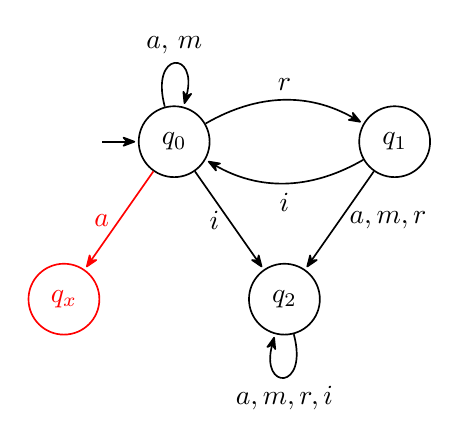
\begin{tikzpicture}[>={Stealth[round]},shorten >=1pt,
                        semithick,initial text=,
                        every state/.style={minimum size=0.9cm}]
      \node[state,initial,visible on=<1->,alt=<8->{accepting}{}]
            (q0) at (0,0)       {$q_0$};
      \node[state,visible on=<4->]  (q1) at (2.8,0)     {$q_1$};
      \node[state,visible on=<5->]  (q2) at (1.4,-2.0)  {$q_2$};
      \node[state,draw=red,text=red,visible on=<2>]
            (qx) at (-1.4,-2.0) {$q_x$};
      \path[->]
        (q0) edge[red,visible on=<2>]         node[left]{$a$}      (qx)
        (q0) edge[loop above,visible on=<3->] node{$a,\,m$}        (q0)
        (q0) edge[bend left,visible on=<4->]  node[above]{$r$}     (q1)
        (q1) edge[bend left,visible on=<6->]  node[below]{$i$}     (q0)
        (q0) edge[visible on=<7->]            node[left]{$i$}      (q2)
        (q1) edge[visible on=<5->]            node[right]{$a,m,r$} (q2)
        (q2) edge[loop below,visible on=<5->] node{$a,m,r,i$}      (q2);
    \end{tikzpicture}}

    \vspace{0.5em}
    {\scriptsize\renewcommand{\arraystretch}{1.2}\setlength{\tabcolsep}{4pt}
    \begin{tabular}{c|cccc|c}
              & $a$ & $m$ & $r$ & $i$ & acc.\\\hline
       $q_0$               & \visible<3->{$q_0$} & \visible<3->{$q_0$} & \visible<4->{$q_1$} & \visible<7->{$q_2$} & \visible<8->{yes}\\
       \visible<4->{$q_1$} & \visible<5->{$q_2$} & \visible<5->{$q_2$} & \visible<5->{$q_2$} & \visible<6->{$q_0$} & \visible<8->{no}\\
       \visible<5->{$q_2$} & \visible<5->{$q_2$} & \visible<5->{$q_2$} & \visible<5->{$q_2$} & \visible<5->{$q_2$} & \visible<8->{no}\\
    \end{tabular}}
  \end{column}

  \begin{column}{0.56\textwidth}
    \small
    \only<1>{%
      \textbf{Initialize.}\\[0.6em]
      Write $s=a{+}m{+}r{\cdot}i$. The start state is the canonical form of the
      regex $s\st$,
      \[
        q_0=[\,s\st\,].
      \]
      Known states: $\{q_0\}$. Now call \texttt{goto} on $q_0$ for each symbol
      $a,m,r,i$.
    }%
    \only<2>{%
      \textbf{\texttt{goto}$(q_0,a)$}
      \begin{align*}
        \Dd_a(s\st)
          &= \Dd_a(s)\cdot s\st\\
          &= \big(\Dd_a(a){+}\Dd_a(m){+}\Dd_a(r)\cdot i\big)\cdot s\st\\
          &= (\eps{+}\emptyset{+}\emptyset\cdot i)\cdot s\st
      \end{align*}
      Left as is, this messy expression is a \alert{brand new state} $q_x$
      (in red). But if we canonicalize it, it folds away.
    }%
    \only<3>{%
      \textbf{Canonicalize}
      \[
        (\eps{+}\emptyset{+}\emptyset\cdot i)\cdot s\st
          \;\sim\; \eps\cdot s\st \;\sim\; s\st = q_0
      \]
      It \textbf{collapses into $q_0$}. Record the self-loop
      $q_0\!\xrightarrow{a}\!q_0$; reading $m$ is identical, so
      $q_0\!\xrightarrow{m}\!q_0$ too. Without canonicalization each such form
      would be a fresh state and the automaton \alert{would never stop
      growing}.
    }%
    \only<4>{%
      \textbf{\texttt{goto}$(q_0,r)$}
      \begin{align*}
        \Dd_r(s\st)
          &= \Dd_r(s)\cdot s\st\\
          &= \big(\emptyset{+}\emptyset{+}\Dd_r(r)\cdot i\big)\cdot s\st\\
          &= (\eps\cdot i)\cdot s\st \;\sim\; i\cdot s\st
      \end{align*}
      A \alert{new} canonical form. Add it as $q_1=i\cdot s\st$, record
      $q_0\!\xrightarrow{r}\!q_1$, and \textbf{recurse into $q_1$}.
    }%
    \only<5>{%
      \textbf{\texttt{goto}$(q_1,a)$, $(q_1,m)$, $(q_1,r)$},\quad
      $q_1=i\cdot s\st$
      \begin{align*}
        \Dd_x(i\cdot s\st)
          &= \Dd_x(i)\cdot s\st + \nu(i)\cdot\Dd_x(s\st)\\
          &= \Dd_x(i)\cdot s\st = \emptyset\cdot s\st \;\sim\; \emptyset
             \quad (x\in\{a,m,r\})
      \end{align*}
      A \alert{new} canonical form $\emptyset$, the \textbf{dead state} $q_2$.
      Add it, record $q_1\!\xrightarrow{a,m,r}\!q_2$, and recurse:
      $\Dd_x(\emptyset)=\emptyset$, so $q_2$ loops to itself on every symbol.
    }%
    \only<6>{%
      \textbf{\texttt{goto}$(q_1,i)$}
      \begin{align*}
        \Dd_i(i\cdot s\st) &= \Dd_i(i)\cdot s\st
                            = \eps\cdot s\st \;\sim\; s\st = q_0
      \end{align*}
      Already known. Record $q_1\!\xrightarrow{i}\!q_0$ and return. $q_1$ is
      done, so we climb back up to $q_0$.
    }%
    \only<7>{%
      \textbf{\texttt{goto}$(q_0,i)$}
      \begin{align*}
        \Dd_i(s\st)
          &= \Dd_i(s)\cdot s\st\\
          &= (\emptyset{+}\emptyset{+}\emptyset\cdot i)\cdot s\st
             \;\sim\; \emptyset = q_2
      \end{align*}
      Already known: the dead state. Record $q_0\!\xrightarrow{i}\!q_2$.
      Reading $i$ with no $r$ before it fails.
    }%
    \only<8>{%
      \textbf{Accepting states and halt}
      \[
        q_0=s\st, \qquad q_1=i\cdot s\st, \qquad q_2=\emptyset.
      \]
      \begin{align*}
        \nu(q_0) &= \eps \;\Rightarrow\; \text{yes}, \quad
        \nu(q_1)  = \emptyset \;\Rightarrow\; \text{no}, \quad
        \nu(q_2)  = \emptyset \;\Rightarrow\; \text{no}
      \end{align*}
      No new canonical form appears, so the construction \alert{halts}. From
      $s\st=(a{+}m{+}r{\cdot}i)\st$ we have built a three-state DFA whose words
      are sequences of the blocks $a$, $m$ and $ri$; for instance it accepts
      \texttt{mariam}. The dead state $q_2$ catches an $i$ with no $r$ before it.
    }%
  \end{column}
\end{columns}
\end{frame}

% =====================================================================
\section{Rocq}

\begin{frame}{Why formalize, and what is Rocq?}
  The derivative theory is easy to state and easy to get subtly wrong: the
  concatenation case, the star case, the finiteness argument. ``This case is
  trivial'' and ``this follows directly'' are exactly where mistakes hide. So we
  machine-check it.
  \vfill
  \textbf{Rocq} (formerly Coq) is an interactive proof assistant: we state each
  theorem and build a proof that a small, \textbf{trusted kernel} verifies
  mechanically, with no step left to take on trust.
  \vfill
  \begin{block}{Used in practice}
    The same tool has checked the CompCert verified C compiler and Gonthier's
    proof of the Four Colour Theorem.
  \end{block}
\end{frame}

\begin{frame}{Type theory and constructive logic}
  Rocq is built on a \textbf{dependent type theory}, the Calculus of Inductive
  Constructions - so its very foundation is a piece of logic.
  \vfill
  \begin{itemize}
    \item By the \textbf{Curry-Howard correspondence}, a proposition is a type
          and a proof is a term of that type, so proving a statement means
          constructing such a term.
    \item Because the logic is \textbf{constructive}, every proof carries
          computational content: a proof that something exists hands you an
          actual witness you can compute with, not merely an assurance that one
          exists.
  \end{itemize}
\end{frame}

\begin{frame}[fragile]{What a proof really is}
  We prove the semantic-syntactic correspondence,
  $w\in\Dd_u(r)\iff u{+}{+}w\in r$. This is the script we write:
  \vfill
  \begin{center}
\begin{lstlisting}[style=rocqstyle,basicstyle=\ttfamily\small]
Lemma D_correct : forall u r w,
  (w \in D u r) = ((u ++ w) \in r).
Proof.
  elim=> [|a u IHu] r w //=.
  rewrite IHu D_char_correct.
  by rewrite -cat_cons.
Qed.
\end{lstlisting}
  \end{center}
  \vfill
  Three tactic lines. They elaborate to the term the kernel actually checks,
  on the next slide.
\end{frame}

\begin{frame}[fragile]{The term the kernel checks}
  What \texttt{Print D\_correct} returns -- no tactics remain:
\begin{lstlisting}[style=rocqstyle,basicstyle=\ttfamily\tiny]
D_correct =
fun _top_assumption_ : word =>
(fun _evar_0_ : (fun l : seq A =>
        forall (r : regex) (w : word), (w \in D l r) = (l ++ w \in r)) [::] =>
   (list_ind
      (fun l : seq A =>
         forall (r : regex) (w : word), (w \in D l r) = (l ++ w \in r))
      _evar_0_)^~ _top_assumption_)
  (fun (r : regex) (w : word) => erefl)
  (fun (a : A) (u : seq A)
       (IHu : forall (r : regex) (w : word), (w \in D u r) = (u ++ w \in r))
       (r : regex) (w : word) =>
     (fun _evar_0_ : (u ++ w \in D_char a r) = (a :: u ++ w \in r) =>
        eq_ind_r (eq^~ (a :: u ++ w \in r)) _evar_0_ (IHu (D_char a r) w))
       ((fun _evar_0_ : (a :: u ++ w \in r) = (a :: u ++ w \in r) =>
           eq_ind_r (eq^~ (a :: u ++ w \in r)) _evar_0_
             (D_char_correct a r (u ++ w)))
          ((fun _evar_0_ : ((a :: u) ++ w \in r) = (a :: u ++ w \in r) =>
              eq_ind ((a :: u) ++ w)
                (fun s : word => (s \in r) = (a :: u ++ w \in r))
                _evar_0_ (a :: u ++ w) (cat_cons a u w))
             erefl)))
\end{lstlisting}
\end{frame}

% =====================================================================
\section{Fuzzy layer}

\begin{frame}{When exact matching is too strict}
  Everything so far rests on one yes-or-no question: are two symbols the
  \emph{very same} symbol? That is often too strict. Real text is noisy -
  symbols get mistyped or swapped for lookalikes, OCR and speech hand us each
  symbol with only a confidence, and in biological sequences chemically close
  bases should count as near matches.
  \vfill
  We would like a pattern to keep matching when the input is merely
  \emph{close} to it, and derivatives to do the same.
  \vfill
  \begin{block}{The question}
    What happens if we keep the crisp derivative theory exactly as it is and
    change one thing -- matching two symbols now means matching \emph{up to
    $\cut$-similarity}?
  \end{block}
\end{frame}

\begin{frame}{Two ways to fuzzify}
  Fuzzifying regular languages is not new, and there are two quite different
  ways to go about it.
  \vfill
  \begin{columns}[T,onlytextwidth]
    \begin{column}{0.47\textwidth}
      The first way puts the fuzziness on \textbf{membership degrees}: a word no
      longer simply belongs to a language, it belongs to a degree in $[0,1]$.
      Some approaches attach a scalar to a regular expression, so that membership
      in its language is scaled by that value.
    \end{column}
    \begin{column}{0.47\textwidth}
      The second way puts it on \textbf{similarity}: we give the symbols a
      similarity relation and extend it to words and languages. Membership stays
      crisp; what softens is the equality underneath it.
    \end{column}
  \end{columns}
  \vfill
  \begin{block}{Why similarity}
    Closeness is a property of the data - the letters, the bases, the sounds -
    not a number we glue onto the language afterwards. Similarity simply replaces
    the exact equality of symbols with a graded notion of closeness.
  \end{block}
\end{frame}

\begin{frame}{Similarity relations on symbols}
  A fuzzy relation grades how close two symbols are,
  $\cR:\Sigma\times\Sigma\to[0,1]$. We ask for two levels of structure.
  \begin{definition}[Proximity and similarity]
    $\cR$ is a \emph{proximity} relation if it is reflexive, $\cR(a,a)=1$, and
    symmetric, $\cR(a,b)=\cR(b,a)$. It is a \emph{similarity} relation if it
    also satisfies the reverse triangle inequality for a T-norm $\otimes$:
    \[
      \cR(a,c)\;\ge\;\cR(a,b)\otimes\cR(b,c).
    \]
  \end{definition}
  A \textbf{T-norm} $\otimes$ generalizes conjunction to $[0,1]$ - commutative,
  associative, monotone, with unit $1$; throughout we take G\"odel's minimum,
  $\otimes=\min$. A \textbf{cut} $\cut\in(0,1]$ turns degrees back into
  yes-or-no through the crisp relation
  $\cR_\cut=\{(a,b)\mid \cR(a,b)\ge\cut\}$.
  \vfill
  \begin{block}{Example}
    $\cR(a,b)=0.9$, $\cR(a,c)=0.2$.
    With cut $\cut=0.8$: $a\sim_\cut b$ since $0.9\ge0.8$, but $a\not\sim_\cut c$.
  \end{block}
\end{frame}

\begin{frame}{From symbols to words and languages}
  The similarity on symbols extends, letter by letter, to words, and then to
  whole languages.
  \begin{definition}[Similarity on words]
    For $w_1=a_1\cdots a_n$ and $w_2=b_1\cdots b_n$ of equal length,
    $\cR^w(w_1,w_2)=\bigotimes_{1\le i\le n} \cR(a_i,b_i)$; for words of
    different length $\cR^w(w_1,w_2)=0$.
  \end{definition}
  \begin{definition}[Similarity on languages]
    \[
      \cR^L(L_1,L_2)=\min\!\Big\{
        \inf_{w_1\in L_1}\sup_{w_2\in L_2}\cR^w(w_1,w_2),\;
        \inf_{w_2\in L_2}\sup_{w_1\in L_1}\cR^w(w_1,w_2)\Big\}.
    \]
  \end{definition}
  Both $\cR^w$ and $\cR^L$ are again similarity relations.
\end{frame}

\begin{frame}{Similarity on expressions}
  Similarity also extends to expressions, comparing two of the \emph{same shape}
  by the similarity of the symbols in corresponding positions.
  \begin{definition}[Similarity on expressions]
    \[
      \cR^E(r_1,r_2)=
      \begin{cases}
        \bigotimes_{1\le i\le n}\cR(a_i,b_i)
          & \text{if } r_1=r[a_1,\dots,a_n]\ \text{and}\ r_2=r[b_1,\dots,b_n];\\[0.4ex]
        0 & \text{otherwise.}
      \end{cases}
    \]
  \end{definition}
  \vfill
  This makes $\cR^E$ \emph{syntax-sensitive}: $a+b$ and $b+a$ denote the
  same language, yet may have $\cR^E(a{+}b,\,b{+}a)=0$.
\end{frame}

\begin{frame}{Shape bounds meaning}
  \small
  Syntactic similarity is always a lower bound on semantic similarity, and the
  semantic value is what you recover by ranging over all expressions with the
  right languages.
  \begin{theorem}[Bridge between $\cR^E$ and $\cR^L$]
    For all restricted regular expressions $r_1,r_2$,
    \[
      \cR^E(r_1,r_2)\ \le\ \cR^L\big(L(r_1),L(r_2)\big),
    \]
    \[
      \cR^L\big(L(r_1),L(r_2)\big)=
      \sup_{\substack{L(r_1)=L(r_1')\\ L(r_2)=L(r_2')}}\cR^E(r_1',r_2').
    \]
  \end{theorem}
  \vfill
  \begin{block}{Example}
    $\cR^E(a{+}b,\,b{+}a)=0$, $\ \cR^L\big(L(a{+}b),L(b{+}a)\big)=1$:
    $\ 0\le 1$.
  \end{block}
  Intersection and complement break this bridge, so the fuzzy theorems live on
  the \textbf{restricted} fragment.
\end{frame}

\begin{frame}{Why the restricted fragment?}
  \small
  A \textbf{restricted} regular expression uses only union, concatenation,
  and star - no intersection ($\wedge$) or complement ($\neg$).
  \vfill
  \begin{block}{Counterexample}
    Let $\cR(a,b)=0.3>0$ for distinct symbols $a,b$. Take
    $r_1=a\wedge a$ and $r_2=a\wedge b$.
    \begin{itemize}
      \item Semantically: $L(r_1)=\{a\}$, $L(r_2)=\{a\}\cap\{b\}=\emptyset$,
        so $\cR^L\big(L(r_1),L(r_2)\big)=0$.
      \item Syntactically, comparing piece by piece:
        $\cR^E(r_1,r_2)=1\otimes\cR(a,b)=0.3$.
    \end{itemize}
  \end{block}
  \vfill
  So $\cR^E(r_1,r_2)=0.3>0=\cR^L\big(L(r_1),L(r_2)\big)$: syntax is no
  longer a lower bound once intersection is allowed - hence the restriction.
\end{frame}

\begin{frame}{Fuzzy derivatives}
  \small
  Now we change matching inside the derivative itself: a symbol counts as read
  when it is $\cut$-similar to the input, not only when it is equal.
  \begin{definition}[Fuzzy language derivative]
    \[
      \partial_a^\cut(L)=\{\,w\mid \exists\,b\in\Sigma,\ \exists\,v\in\Sigma^*:\
        \cR(a,b)\otimes\cR^w(w,v)\ge\cut,\ bv\in L\,\}.
    \]
  \end{definition}
  \begin{definition}[Fuzzy expression derivative]
    \[
      \Dd_a^\cut(r)=\!\!\sum_{\cR(a,b)\otimes\cR^E(s,r)\ge\cut}\!\!\Dd_b(s),
    \]
    a \emph{finite} sum of ordinary Brzozowski derivatives, since only finitely
    many $s$ satisfy $\cR^E(s,r)\neq0$ when $\Sigma$ is finite.
  \end{definition}
  \begin{theorem}[Regularity is preserved]
    If $L$ is regular then $\partial_a^\cut(L)$ is regular; if $r$ is a
    restricted expression then $\Dd_a^\cut(r)$ is again a restricted expression.
  \end{theorem}
\end{frame}

\begin{frame}{G\"odel's min: fuzzy = crisp over a quotient}
  With G\"odel's minimum the cut relation
  $a\sim_\cut^\Sigma b \iff \cR(a,b)\ge\cut$ is not only reflexive and symmetric
  but \textbf{transitive}, so it is an \emph{equivalence}. We may then bundle
  $\cut$-similar symbols into classes.
  \begin{definition}[Quotient alphabet]
    $\Sigma^\cut=\Sigma/{\sim_\cut^\Sigma}$, with quotient map
    $q_\cut(a)=[a]_\cut$, extended to words by $q_\cut^*$, and image
    $L^\cut=q_\cut^*(L)$.
  \end{definition}
  \begin{theorem}[Reduction to the quotient alphabet]
    A fuzzy derivative over $\Sigma$ is exactly an ordinary derivative over the
    quotient alphabet $\Sigma^\cut$:
    \[
      \partial_a^\cut(L)=\{\,w\mid q_\cut^*(w)\in\partial_{[a]_\cut}(L^\cut)\,\},
      \qquad
      q_\cut^*\big(\partial_a^\cut(L)\big)=\partial_{[a]_\cut}\big(L^\cut\big).
    \]
  \end{theorem}
\end{frame}

\begin{frame}{Everything carries over}
  Because the fuzzy theory is just the crisp theory read over $\Sigma^\cut$,
  each earlier result transfers.
  \begin{itemize}
    \item \textbf{Fuzzy interpretation:}
      $\ \mathcal L^\cut(r)=\{\,w\mid w\sim_\cut^{\Sigma^*}v\ \text{for some}\ v\in L(r)\,\}$.
    \item \textbf{Correspondence:}
      $\ \mathcal L^\cut\big(\Dd_u^\cut(r)\big)=\partial_u^\cut\big(L(r)\big)$.
    \item \textbf{Finiteness:} $\ \{\partial_u^\cut(L)\mid u\in\Sigma^*\}$ is finite.
    \item \textbf{Fuzzy automaton:} $\ \mathcal L(M^\cut)=\mathcal L_\Sigma^\cut(r)$,
      the words $\cut$-close to some word of $r$.
  \end{itemize}
  \vfill
  And the quotient transition reads back as a \textbf{fuzzy
  transition}: $\delta(q_1,[a])=q_2$ holds with membership degree $\cut$.
\end{frame}

% =====================================================================
\section{Conclusion}

\begin{frame}{Conclusion}
  \textbf{What we have shown.}
  \begin{itemize}
    \item The classical derivative theory, up to DFA correctness, is
          formalized in Rocq.
    \item We fuzzify through \textbf{similarity on symbols} rather than
          membership degrees.
    \item The \textbf{quotient alphabet} $\Sigma^\cut$ reduces the fuzzy theory
          to the crisp one, so every earlier result carries over unchanged.
  \end{itemize}
  \medskip
  \textbf{Future work.}
  \begin{itemize}
    \item Formalize the \textbf{fuzzy layer} in Rocq.
    \item \textbf{Constructive finiteness}: a Kuratowski-finiteness result via
          normalized representatives.
    \item Generalize beyond G\"odel's $\min$ to a \textbf{general T-norm}.
  \end{itemize}
\end{frame}

\begin{frame}
  \vfill
  \begin{center}
    {\Huge Thank you}\\[0.6em]
    {\large Questions?}
  \end{center}
  \vfill
\end{frame}

\end{document}
